%
%Free under Creative Commons Attribution-NonCommercial 4.0 International (CC BY-NC 4.0)
%


\documentclass[12pt]{article}
\usepackage{fancyhdr}
\usepackage{color}
\usepackage{multicol}
\usepackage{enumitem}
\usepackage{graphicx}
\usepackage{sectsty}
\usepackage{array}
\usepackage{tikz}
\usepackage{tkz-euclide}
\usepackage[first=2, last=13]{lcg}

\allsectionsfont{\centering}

\pagestyle{empty}

\usepackage{draftwatermark}
	\SetWatermarkText{\copyright wolf-math.com}
	\SetWatermarkScale{4}
	\SetWatermarkLightness{1}

\usepackage[margin=1in, headsep=0pt]{geometry}
\setlength{\parindent}{0cm}


\begin{document}
\setcounter{secnumdepth}{-1}

Mr. Wolf \\ wolf-math.com

\newcommand{\random}{\rand\arabic{rand}}

\section{Rational Exponents \& Radicals}



\textbf{SWBAT} simplify exponential expressions by properly using properties of exponents.\\

\textbf{SWBAT} simplify radical expressions by factoring out primes of the radicand.\\
	
\textbf{SWBAT} simplify radical expressions using properties of radicals.\\

\textbf{SWBAT} convert from radical form to rational exponent form.\\
	
\textbf{SWBAT} simplify rational exponents using properties of exponents\\
	
\textbf{SWBAT} evaluate rational exponential expressions by breaking them apart into the product property.\\
	
\textbf{SWBAT} solve a square root equation.\\

\textbf{SWBAT} solve a radical equation with index $>2$.\\

\textbf{SWBAT} identify extraneous solutions of radical equations.\\

\textbf{SWBAT} solve an equation that has an exponent by using the reciprocal exponent as the inverse function.\\

\textbf{SWBAT} identify exponential functions, and differentiate between exponential and power functions.\\

\textbf{SWBAT} graph exponential functions by using a t-chart.\\

\textbf{SWBAT} graph exponential functions without using a t-chart.\\

\textbf{SWBAT} determine the end behavior of an exponential function.\\

\textbf{SWBAT} identify translations of the exponential graph by identifying key parts of the equation.\\

\textbf{SWBAT} calculate compound interest given the interest rate, number of years, and number of times per year, and the principal.\\

\textbf{SWBAT} use the number $e$ as an exponential base for continuously compounded interest.\\
	


\subsection{Standards}
	\textbf{Real Number System \hfill N-RN.1}\\
	
	 Explain how the definition of the meaning of rational exponents follows from extending the properties of integer exponents to those values, allowing for a notation for radicals in terms of rational exponents. For example, we define $5^{\frac{1}{3}}$ to be the cube root of 5 because we want $\left(5^{\frac{1}{3}}\right)^{3} =\left(5^{\frac{1}{3}}\right)^{3}$ to hold, so $\left(5^{\frac{1}{3}}\right)^{3}$ must equal 5. \\
	
2.	 Rewrite expressions involving radicals and rational exponents using the properties of exponents.
	

\textbf{Creating Equations A -CED} Create equations that describe numbers or relationships\\

1. Create equations and inequalities in one variable and use them to solve problems. Include equations arising from linear and quadratic functions, and simple rational and exponential functions.\\

\textbf{Interpreting Functions F-IF} Analyze functions using different representations \\

7. Graph functions expressed symbolically and show key features of the graph, by hand in simple cases and using technology for more complicated cases.\\

e. Graph exponential and logarithmic functions, showing intercepts and end behavior, and trigonometric functions, showing period, midline, and amplitude.\\

\subsection{Pre-Assessment} To introduce our topic of exponential functions the students will begin by learning properties of exponents. The students should have already encountered this before, but since this information is necessary for our topic we will review the content and make sure that there are absolutely no misconceptions.  
	


\subsection{Assessments} Homework will be graded, there will be a lab, and test on this material. 
	


\subsection{Before \& After}

	\textbf{Before} the students learned about creating algebraic expressions that represent a rule. This lesson prepares students for the extention of those that we just learned in our first unit. While we were learning about arithmetic functions before, we are now moving towards exponential functions.\\
	


	\textbf{After} we will be learning how to solve for an exponential expression. This requires knowledge of the properties of exponents and rational exponents. From there we will analyze and model exponential functions.
	

\subsection{Connections}



\let\stdsection\section
\renewcommand\section{\newpage\stdsection}

\section{Pre-Assessment}



\section{Properties of Exponents}


\begin{enumerate}
\setlength\itemsep{1cm}

	\item \textbf{Product Property:} $a^m \cdot a^n= a^{m+n}$\hspace{1cm} \textbf{and} \hspace{1cm} $(xy)^m=x^m \cdot y^m$ \\
	
		\hspace{.6in} Example: $2^6 \cdot 2^8=2^{14}$\hspace{1cm}   \textbf{ and}  \hspace{1cm}  $(2x)^{5}=2^5 \cdot x^5$\\ 
	
	\item \textbf{Power Property:} $\left(a^m \right)^n = a^{(m \cdot n)}$\\
	
		\hspace{.6in} Example: $\left(g^2\right)^3=g^6$\\ 
	
	\item \textbf{Quotient Property:} $\frac{a^m}{a^n}=a^{m-n}$\\
	
		\hspace{.6in} Example: $\frac{k^7}{k^4} = k^3$ and $\frac{k^2}{k^8}=k^{-6}$\\ 
	
	\item \textbf{Negative Property:} $a^{-n}=\frac{1}{a^n}$ and $\frac{1}{a^{-n}}=a^{n}$ \\
	
		\hspace{.6in} Example: $2^{-1}=\frac{1}{2}$\hspace{1cm} \textbf{and} \hspace{1cm} $\left(\frac{1}{2}\right)^{-1}=2$ \hspace{1cm} \textbf{and} \hspace{1cm} $\left(\frac{2}{3}\right)^{-1}=\frac{3}{2}$\\ 
	
	\item \textbf{Zero Property:} $a^0=1$\\
		
		\hspace{.6in} Example: $555,987,123,987,123^0=1$\\ 
	
	\item \textbf{Power of a Quotient Property:} $\left(\frac{a}{b}\right)^n=\frac{a^n}{b^n}$\\
	
		\hspace{.6in} Example: $\left(\frac{2}{3}\right)^3=\frac{2^3}{3^3}=\frac{8}{27}$ \\

\end{enumerate}

\pagebreak

\section{Properties of Exponents -- Notes}


\begin{enumerate}
\setlength\itemsep{1cm}

	\item \textbf{Product Property:} \\
	
		\hspace{.6in} Example: \\ 
	
	\item \textbf{Power Property:} \\
	
		\hspace{.6in} Example: \\ 
	
	\item \textbf{Quotient Property:} \\
	
		\hspace{.6in} Example: \\ 
	
	\item \textbf{Negative Property:} \\
	
		\hspace{.6in} Example:\\ 
	
	\item \textbf{Zero Property:} \\
		
		\hspace{.6in} Example:\\ 
	
	\item \textbf{Power of a Quotient Property:}\\
	
		\hspace{.6in} Example: \\

\end{enumerate}

\pagebreak

\subsection{Board Work}

Simplify each expression.\\

\begin{enumerate}

	\item $f^3 \cdot f^5=$\\
	
	\item $7^3 \cdot 7^7=$\\
	
	\item $(bc)^5=$\\
	
	\item $(2g)^3=$\\
	
	\item $(u^9)^{10}=$\\
	
	\item $ (4^2)^5=$\\
	
	\item $\frac{v^8}{v^2}=$\\
	
	\item $\frac{v^2}{v^8}=$\\
	
	\item $\left(\frac{2}{3}\right)^4=$\\
	
	\item $q^{-1}=$\\
	
	\item $6^{-3}=$\\
	
	\vspace{1cm}
	
	Challenge problem: $\frac{9x^2y^3z^{2}}{3xy^{-5}z^{6}}=$\\

\end{enumerate}	
	
\pagebreak

\subsection{You Try: Partner Work}


\textbf{Section 1: Multiplication--} Simplify each product of exponents. Leave answers in exponential form.\\

Example 1: $x^5 \cdot x^2=x^7$\\

\begin{enumerate}
\begin{multicols}{2}

	\item $ y^6 \cdot y^4 =\underline{\hspace{1in}}$\\
	
	\item $(7h)^3=\underline{\hspace{1in}}$\\
	
	\item $ 5^{3} \cdot (5n)^2=\underline{\hspace{1in}}$\\
	
	\item $ (2n)^{3} \cdot 2^2 = \underline{\hspace{1in}}$\\

\end{multicols}
\end{enumerate}


\hrulefill

\textbf{Section 2: Fractions \& division -- } Simplify each expression. Make sure there are no negative exponents. Leave answers in exponential form.\\ 

\begin{enumerate}[resume]
\begin{multicols}{2}

	\item $\left(\frac{1}{n}\right)^{3}=\underline{\hspace{1in}}$\\
	
	\item $\frac{p^6}{p^3}=\underline{\hspace{1in}}$\\
	
	\item $\frac{h^9}{h^{12}}=\underline{\hspace{1in}}$\\
	
	\item $\left(\frac{2^2m^3n^{2}}{2mn^2}\right)=\underline{\hspace{1in}}$\\

\end{multicols}
\end{enumerate}

\hrulefill

\textbf{Section 3: Negative and Zero Exponents --} Simplify each expression so that there are no negative exponents. Leave answers in exponential form.

\begin{enumerate}[resume]
\begin{multicols}{2}

	\item $6^{-2}=\underline{\hspace{1in}}$\\

	\item $(bagillion)^0=\underline{\hspace{1in}}$\\
	
	\item $\left(\frac{1}{10}\right)^{-3}=\underline{\hspace{1in}}$\\
	
	\item $\left(\frac{7}{2}\right)^{2}=\underline{\hspace{1in}}$\\
	
	
\end{multicols}
\end{enumerate}

\hrulefill

\textbf{Section 4: Powers of exponents--} Simplify so that there is only one level of exponent (e.g. \textbf{don't} write $2^{2^2}$ as an answer). Leave answers in exponential form.

\begin{enumerate}[resume]
\begin{multicols}{2}

	\item $\left(2^2\right)^2=\underline{\hspace{1in}}$\\
	
	\item $\left(c^5\right)^7=\underline{\hspace{1in}}$\\
	
	\item $\left(\frac{1}{2}\right)^{10}=\underline{\hspace{1in}}$\\
	
	\item $\left(\left(\frac{3}{4}\right)^{-1}\right)^{-1}=\underline{\hspace{1in}}$\\

\end{multicols}
\end{enumerate}

\pagebreak

\section{Square Roots}

Square Roots are the opposite of squares (exponent of 2). This is also called an \textit{inverse}.\\

\begin{LARGE}
	$$\sqrt{a^2}=a$$
\end{LARGE}



\hrulefill

There are 2 parts to a squareroot.

\begin{enumerate}

	\item the \textit{RADICAL}\\
	
	\item the \textit{RADICAND}\\
	
\end{enumerate}

\begin{center}
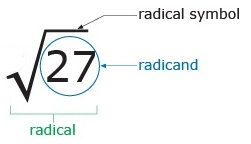
\includegraphics[scale=.7]{squareroot.jpg}
\end{center}


The \textit{radical} tells us that we're looking for identical factors.\\

the \textit{radicand} is a number that needs to be factored so we can pull out the identical ones.\\

\textbf{Example:} $\sqrt{25}=\sqrt{5\cdot5} \Longrightarrow$ since there are 2 5's $\Longrightarrow \sqrt{5\cdot5}=5$\\

\pagebreak

\section{Simplifying Square Root Expressions}

\begin{center}
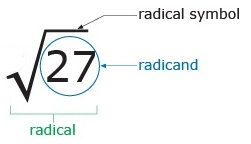
\includegraphics[scale=.7]{squareroot.jpg}\\
\end{center}

To simplify radical expressions follow these steps\\

\textbf{Step 1:} factor the radicand\\

\textbf{Step 2:} pull out factors that a repeated twice.\\

\textbf{Step 3:} all other factors stay inside the radical\\

\hrulefill

\textbf{Examples:} Simplify the square root.\\

\begin{multicols}{2}
\textbf{We try:}\\

\begin{enumerate}
	\setlength\itemsep{1cm}

	\item $\sqrt{36}$\\
	
	
	\item $\sqrt{50}$\\
	
	
	\item $\sqrt{27}$\\
	
	
	\item $\sqrt{27x^2}$\\
	
		
\textbf{You Try:}\\
	
	\item  $\sqrt{120}$ \\
	
	
	\item $\sqrt{52y^4}$\\
	
	
	\item $\sqrt{16}$\\
	
	
	\item $\sqrt{160n^7}$\\
	
	

\end{enumerate}
\end{multicols}

 \textbf{Challenge Problem:} $\sqrt[5]{800h^{11}}$
 

\pagebreak

\subsection{Simplifying Square Root Expressions-- Guided Notes}

\begin{center}
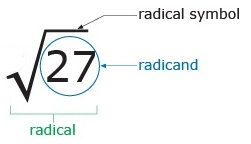
\includegraphics[scale=.7]{squareroot.jpg}\\
\end{center}

To simplify radical expressions follow these steps\\

\textbf{Step 1:} \\

\textbf{Step 2:} \\

\textbf{Step 3:} \\

\hrulefill

\textbf{Examples:} Simplify the square root.\\

\begin{multicols}{2}
\textbf{We try:}\\

\begin{enumerate}
	\setlength\itemsep{1cm}

	\item $\sqrt{36}$\\
	
	
	\item $\sqrt{50}$\\
	
	
	\item $\sqrt{27}$\\
	
	
	\item $\sqrt{27x^2}$\\
	
		
\textbf{You Try:}\\
	
	\item  $\sqrt{120}$ \\
	
	
	\item $\sqrt{52y^4}$\\
	
	
	\item $\sqrt{16}$\\
	
	
	\item $\sqrt{160n^7}$\\
	
	

\end{enumerate}
\end{multicols}


\section{Other Roots}

Roots are the opposite of exponents. This is also called an \textit{inverse}.\\

\begin{LARGE}
	$$\sqrt[n]{a^n}=a$$
\end{LARGE}



\hrulefill

There are \textit{actually} 3 parts to a radical. Square-roots don't have an index because we assume it's 2.

\begin{enumerate}

	\item the \textit{RADICAL}\\
	
	\item the \textit{RADICAND}\\
	
	\item the \textit{INDEX}\\
\end{enumerate}

\begin{center}
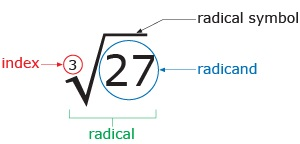
\includegraphics[scale=.7]{radical.jpg}
\end{center}



The \textbf{radical} tells us that we're looking for identical factors.\\

The \textbf{index} tells us how many identical factors we're looking for.\\

the \textbf{radicand} is a number that needs to be factored so we can pull out the identical ones.\\

\textbf{Example:} $\sqrt[3]{125}=\sqrt{5\cdot5\cdot 5} \Longrightarrow$ since the index is 3, and there are 3- 5's $\Longrightarrow \sqrt[3]{5\cdot5\cdot5}=5$\\

\pagebreak

\section{Simplifying Radical Expressions}

\begin{center}
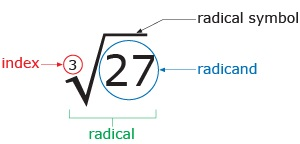
\includegraphics[scale=.7]{radical.jpg}\\
\end{center}

To simplify radical expressions follow these steps\\

\textbf{Step 1:} determine the index\\

\textbf{Step 2:} factor the radicand\\

\textbf{Step 3:} pull out repeated factors of the amount of the index\\

\textbf{Step 4:} all other factors stay inside the radical\\

\textbf{Examples:} Simplify the radical, keep track of the index\\

\begin{multicols}{2}
\textbf{We try:}\\

\begin{enumerate}
	\setlength\itemsep{1cm}

	\item $\sqrt[3]{8}$\\
	
	
	\item $\sqrt[4]{48}$\\
	
	
	\item $\sqrt[3]{27}$\\
	
	
	\item $\sqrt[3]{27x^5}$\\
	
		
\textbf{You Try:}\\
	
	\item  $\sqrt[3]{120}$ \\
	
	
	\item $\sqrt[4]{162y^4}$\\
	
	
	\item $\sqrt[4]{32}$\\
	
	
	\item $\sqrt[3]{162n^7}$\\
	
	

\end{enumerate}
\end{multicols}

 \textbf{Challenge Problem:} $\sqrt[5]{800h^{11}}$
 
 \section{Other Roots-- Guided Notes}

Roots are the opposite of exponents. This is also called an \textit{inverse}.\\

\begin{LARGE}
	$$\sqrt[n]{a^n}=a$$
\end{LARGE}



\hrulefill

There are \textit{actually} 3 parts to a radical. Square-roots don't have an index because we assume it's 2.

\begin{enumerate}

	\item the \\
	
	\item the \\
	
	\item the\\
\end{enumerate}

\begin{center}
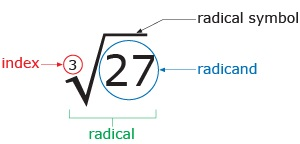
\includegraphics[scale=.7]{radical.jpg}
\end{center}



The \textbf{radical} \\

The \\

the \\

\textbf{Example:} $\sqrt[3]{125}=$\\

\pagebreak

\section{Simplifying Radical Expressions -- Guided Notes}

\begin{center}
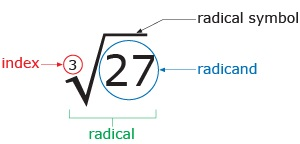
\includegraphics[scale=.7]{radical.jpg}\\
\end{center}

To simplify radical expressions follow these steps\\

\textbf{Step 1:} \\

\textbf{Step 2:} \\

\textbf{Step 3:} \\

\textbf{Step 4:} \\

\textbf{Examples:} Simplify the radical, keep track of the index\\

\begin{multicols}{2}
\textbf{We try:}\\

\begin{enumerate}
	\setlength\itemsep{1cm}

	\item $\sqrt[3]{8}$\\
	
	
	\item $\sqrt[4]{48}$\\
	
	
	\item $\sqrt[3]{27}$\\
	
	
	\item $\sqrt[3]{27x^5}$\\
	
		
\textbf{You Try:}\\
	
	\item  $\sqrt[3]{120}$ \\
	
	
	\item $\sqrt[4]{162y^4}$\\
	
	
	\item $\sqrt[4]{32}$\\
	
	
	\item $\sqrt[3]{162n^7}$\\
	
	

\end{enumerate}
\end{multicols}

 \textbf{Challenge Problem:} $\sqrt[5]{800h^{11}}$

\section{Add \& Subtract Radical Expressions}

When adding and subtracting radical expressions, treat the radical like a variable whenever possible.\\

$$\sqrt{a} + \sqrt{a} = 2\sqrt{a}$$

The roots need to be exactly the same (i.e. same index, same radicand) to be able to add or subtract.\\

\textbf{Example 1:} $5\sqrt{7} - 3 \sqrt{7} = 2\sqrt{7}$\\

\vspace{1cm}

Sometimes the radical needs to be simplified before adding or subtracting.\\

\textbf{Example 2:} $\sqrt{3} + \sqrt{12}=$\\

\vspace{1cm}

\hrulefill

\textbf{You Try:}\\

\begin{enumerate}
\setlength\itemsep{1cm}

	\item $8\sqrt{h}+ 9\sqrt{h}=$\\
	
	\item $2\sqrt{x} - \sqrt{x}=$\\
	
	\item $6\sqrt{p} - 10 \sqrt{p}=$\\
	
	\item $\sqrt[3]{81} + \sqrt[3]{3}=$\\
	
	\item $\sqrt{8} + \sqrt{32} - \sqrt{2}=$\\
	
\end{enumerate}

\section{Multiplication \& Division with Radical Expressions}

If two roots (with the same index) are multiplied, just multiply the inside numbers. 

$$\sqrt{a} \cdot \sqrt{b} = \sqrt{a \cdot b}$$

$$\sqrt{a \cdot b}= \sqrt{a}\cdot \sqrt{b}$$

\textbf{Example 1:} $\sqrt[5]{8} \cdot \sqrt[5]{4}=$\\

\vspace{1cm}

\textbf{Example 2:} $3\sqrt{5} \cdot 4 \sqrt{6}=$\\

\vspace{1cm}

\textbf{Example 3:} $(2+\sqrt{h})(5+\sqrt{h})=$\\

\vspace{.7cm}

\hrulefill

Dividing is just as easy. The square-root symbol can be either broken or put together to the top and bottom.
	
$$\sqrt{\frac{a}{b}}= \frac{\sqrt{a}}{\sqrt{b}}$$

\textbf{Example 3:} $\sqrt{\frac{16}{25}}=$

\vspace{1cm}

\textbf{Example 4:} $\sqrt{\frac{8}{100}}=$

\vspace{.7cm}


\hrulefill

\textbf{You Try:}
\begin{enumerate}
\begin{multicols}{2}
\setlength\itemsep{1cm}

	\item $\sqrt{10} \cdot \sqrt{10}=$\\
	
	\item $\sqrt{12} \cdot \sqrt{4}=$\\
	
	\item $(-1 + \sqrt{3})(8 - \sqrt{6})=$\\
	
	\item $\sqrt{\frac{3}{4}}=$\\
	
	\item $\sqrt{\frac{9}{4}}=$\\
	
	\item $\sqrt{\frac{25}{75}}=$
\end{multicols}
\end{enumerate} 

\section{Add \& Subtract Radical Expressions -- Guided Notes}

When adding and subtracting radical expressions, treat the radical like a variable whenever possible.\\

$$\sqrt{a} + \sqrt{a} =$$

The roots need to be exactly the same (i.e. same index, same radicand) to be able to add or subtract.\\

\textbf{Example 1:} $5\sqrt{7} - 3 \sqrt{7} = $\\

\vspace{1cm}

Sometimes the radical needs to be simplified before adding or subtracting.\\

\textbf{Example 2:} $\sqrt{3} + \sqrt{12}=$\\

\vspace{1cm}

\hrulefill

\textbf{You Try:}\\

\begin{enumerate}
\setlength\itemsep{1cm}

	\item $8\sqrt{h}+ 9\sqrt{h}=$\\
	
	\item $2\sqrt{x} - \sqrt{x}=$\\
	
	\item $6\sqrt{p} - 10 \sqrt{p}=$\\
	
	\item $\sqrt[3]{81} + \sqrt[3]{3}=$\\
	
	\item $\sqrt{8} + \sqrt{32} - \sqrt{2}=$\\
	
\end{enumerate}

\section{Multiplication \& Division with Radical Expressions -- Guided Notes}

If two roots (with the same index) are multiplied, just multiply the inside numbers. 

$$\sqrt{a} \cdot \sqrt{b} = $$

$$\sqrt{a \cdot b}= $$

\textbf{Example 1:} $\sqrt[5]{8} \cdot \sqrt[5]{4}=$\\

\vspace{.7cm}

\textbf{Example 2:} $3\sqrt{5} \cdot 4 \sqrt{6}=$\\

\vspace{.7cm}

\textbf{Example 3:} $(2+\sqrt{h})(5+\sqrt{h})=$\\

\vspace{.7cm}

\hrulefill

Dividing is just as easy. The square-root symbol can be either broken or put together to the top and bottom.
	
$$\sqrt{\frac{a}{b}}= \frac{\sqrt{a}}{\sqrt{b}}$$

\textbf{Example 3:} $\sqrt{\frac{16}{25}}=$

\vspace{.7cm}

\textbf{Example 4:} $\sqrt{\frac{8}{100}}=$

\vspace{.7cm}


\hrulefill

\textbf{You Try:}
\begin{enumerate}
\begin{multicols}{2}
\setlength\itemsep{1cm}

	\item $\sqrt{10} \cdot \sqrt{10}=$\\
	
	\item $\sqrt{12} \cdot \sqrt{4}=$\\
	
	\item $(-1 + \sqrt{3})(8 - \sqrt{6})=$\\
	
	\item $\sqrt{\frac{3}{4}}=$\\
	
	\item $\sqrt{\frac{9}{4}}=$\\
	
	\item $\sqrt{\frac{25}{75}}=$
\end{multicols}
\end{enumerate} 

\section{Rational Exponents}

Rational = Fraction \\

What does it mean to have a fraction in the exponent?\\

\begin{center}
\begin{tikzpicture}[scale=2.5]

	\draw (0,0) -- (2,0) -- (2,2) -- (0,2) -- cycle;
	\node at (1,1){area=$a$};
	\node at (1,-.2){$\sqrt{a}$};
	\node at (-.2,1){$\sqrt{a}$};
	

\end{tikzpicture}
\end{center}

%\begin{center}
%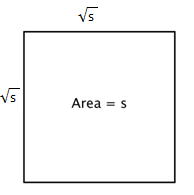
\includegraphics[scale=1]{square.png}
%\end{center}

Area of a square $=($side length$)^2$.\\

This makes sense because $a=\sqrt{a} \sqrt{a} = \sqrt{a^2}$\\

(or $a=\sqrt{a} \sqrt{a} = (\sqrt{a})^2$ they're both the same.)\\

Using our \textbf{product property of exponents}, which power, when added to itself is 1? $$a=a^{\frac{1}{2}} \cdot a^{\frac{1}{2}}=\left(a^{\frac{1}{2}}\right)^2$$ since we add the exponents. From here we learn that $\sqrt{a}=a^{\frac{1}{2}}$\\

Having a fraction in the exponent is called a \textbf{RATIONAL EXPONENT.} A \textit{rational exponent} is just another way to write a root. 

\begin{large}
	$$\sqrt{n}= n^{\frac{1}{2}}$$

\end{large}


or more generically, for any index $a$\\

\begin{large}

	$$\sqrt[a]{n^b}=n^{\frac{b}{a}}$$ 
	
\end{large}



\pagebreak

\section{Rational Exponents -- Guided Notes}

Rational = Fraction \\

What does it mean to have a fraction in the exponent?\\

\begin{center}
\begin{tikzpicture}[scale=2.5]

	\draw (0,0) -- (2,0) -- (2,2) -- (0,2) -- cycle;
	\node at (1,1){area=$a$};
	\node at (1,-.2){$\sqrt{a}$};
	\node at (-.2,1){$\sqrt{a}$};
	

\end{tikzpicture}
\end{center}

%\begin{center}
%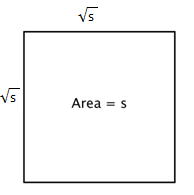
\includegraphics[scale=1]{square.png}
%\end{center}

Area of a square $=($side length$)^2$.\\

This makes sense because $a=$\\

(or $a=$ \hspace{3in} they're both the same.)\\

Using our \textbf{product property of exponents}, which power, when added to itself is 1? $$a=$$\\

Having a fraction in the exponent is called a \textbf{RATIONAL EXPONENT.} A \textit{rational exponent} is just another way to write a root. 

\begin{large}
	$$\sqrt{n}= $$

\end{large}


or more generically, for any index $a$\\

\begin{large}

	$$\sqrt[]{\hspace{1cm}}=n$$ 
	
\end{large}



OMG that looks scary...

\pagebreak

\section{Rational Exponents -- What's the point?}

\begin{enumerate}

\item It's more natural given what we know about roots and their inverses.\\

\item For the sake of exponential functions.\\

\item Sometimes calculators have an exponent button, but no root button $index>3$.\\

\item \begin{verbatim}Intentionally left blank for student response.
\end{verbatim}
\end{enumerate}





\textbf{Board Work:} Convert the following from radical form into rational exponent form.\\

\begin{enumerate}
\setlength\itemsep{.4cm}

\item $\sqrt[3]{9^2}=$\\ 

\item $\sqrt[6]{j^5}=$\\

\item $\sqrt[10]{3^3 \cdot k^7}=$\\
\end{enumerate}

\hrulefill

\textbf{You Try:} Convert the following radical expressions into rational exponent expressions.\\

\begin{enumerate}
\begin{multicols}{2}
\setlength\itemsep{1cm}
\item $\sqrt{7}=$

\item $\sqrt{h^3}=$

\item $\sqrt[3]{27j^3}=$

\item $\sqrt[5]{k^{10}}=$


\end{multicols}
\end{enumerate}

\hrulefill

\textbf{You Try:} Convert the rational exponent into a radical -- You don't need to simplify

\begin{enumerate}[resume]
\begin{multicols}{2}
\setlength\itemsep{1cm}
\item $8^{\frac{1}{2}}=$

\item $3^{\frac{7}{8}}=$

\item $(5h)^{\frac{3}{2}}=$

\item $(10k^2)^{\frac{1}{3}}=$

\end{multicols}
\end{enumerate}

\hrulefill

\textbf{You Try:} Create your own rational exponent conversion. Make there is a number base and a variable base with and index$>1$, and an exponent$>1$.





\section{Simplifying Rational Exponential Expressions}
Use the properties of exponents to convert, and simplify the radicals and rational exponents. \\

\textbf{The Product Property:} $a^m\cdot a^n=a^{(m+n)}$\\

\hspace{1in} $8^{\frac{1}{2}} \cdot  8^{\frac{3}{2}}=$\\

\vspace{1cm}

\textbf{The Product Property 2:} $(a\cdot b)^m=a^m\cdot b^m$\\

\hspace{1in}$\left(5x\right)^{\frac{3}{2}}=$\\

\vspace{1cm}

\textbf{The Power Property:} $\left(a^m\right)^{n}=a^{(m\cdot n)}$\\

\hspace{1in} $\left(h^{\frac{5}{7}}\right)^{\frac{6}{5}}=$\\

\vspace{1cm}

\textbf{The Quotient Property:} $\frac{a^m}{a^n}=a^{m-n}$\\

\hspace{1in} $\left(\frac{3^{\frac{3}{2}}}{3^{\frac{1}{2}}}\right)=$\\

\vspace{1cm}

\textbf{The Negative Property:} $a^{-b}=\frac{1}{a^{b}}$ \hspace{1cm} or \hspace{1cm} $\frac{1}{a^{-b}}=a^b$\\

\hspace{1in} $(81)^{-\frac{1}{2}}=$\\

\vspace{1cm}

\textbf{Power of a Quotient Property:} $\left(\frac{a}{b}\right)^c=\frac{a^c}{b^c}$\\

\hspace{1in} $\left(\frac{9}{4}\right)^{\frac{1}{2}}=$\\

\vspace{1cm}


\pagebreak

\section{Evaluating Rational Exponents}

3-Step process for evaluating rational exponential expressions. $a^{\frac{m}{n}}$

\begin{enumerate}

	\item Factor the base of the exponent 
	
	\item Determine the ratio of bases $\frac{m}{n}$
	
	\item Pull out the ratio amount of the bases. 

\end{enumerate}

\textbf{Example:} $\left(216\right)^{\frac{2}{3}}$\\

	\begin{enumerate}
	
		\item $\left(216\right)^{\frac{2}{3}}= \left( 2 \cdot 2 \cdot 2 \cdot 3 \cdot 3 \cdot 3\right)^{\frac{2}{3}}$\\
		
		\item Ratio = $\frac{2}{3}$\\
		
		\item Pull out $\frac{2}{3}$ of each factor  -- $\left( 2 \cdot 2 \cdot 2 \cdot 3 \cdot 3 \cdot 3\right)^{\frac{2}{3}}= 2 \cdot 2 \cdot 3 \cdot 3 = 36$
	
	
	\end{enumerate}

\hrulefill

\textbf{You Try:} Evaluate the rational exponential expressions. Keep an eye out for properties of exponents.\\

\begin{multicols}{2}
\begin{enumerate}
		\setlength\itemsep{1cm}

\item $25^{\frac{1}{2}}$\\

\item $1000^{\frac{2}{3}}$\\

\item $121^{\frac{3}{2}}$\\

\item $49^{-\frac{1}{2}}$\\

\item  $32^{\frac{3}{5}}$\\

\item $16^{-\frac{-5}{2}}$\\

\item $0.04^{\frac{1}{2}}$\\

\item $\left(\frac{1}{125}\right)^{-\frac{1}{3}}$

\end{enumerate}
\end{multicols}

\pagebreak

\section{Simplifying Rational Exponential Expressions}
Use the properties of exponents to convert, and simplify the radicals and rational exponents. \\

\textbf{The Product Property:} $a^m\cdot a^n=a^{(m+n)}$\\

\hspace{1in} $8^{\frac{1}{2}} \cdot  8^{\frac{3}{2}}=$\\

\vspace{1cm}

\textbf{The Product Property 2:} $(a\cdot b)^m=a^m\cdot b^m$\\

\hspace{1in}$\left(5x\right)^{\frac{3}{2}}=$\\

\vspace{1cm}

\textbf{The Power Property:} $\left(a^m\right)^{n}=a^{(m\cdot n)}$\\

\hspace{1in} $\left(h^{\frac{5}{7}}\right)^{\frac{6}{5}}=$\\

\vspace{1cm}

\textbf{The Quotient Property:} $\frac{a^m}{a^n}=a^{m-n}$\\

\hspace{1in} $\left(\frac{3^{\frac{3}{2}}}{3^{\frac{1}{2}}}\right)=$\\

\vspace{1cm}

\textbf{The Negative Property:} $a^{-b}=\frac{1}{a^{b}}$ \hspace{1cm} or \hspace{1cm} $\frac{1}{a^{-b}}=a^b$\\

\hspace{1in} $(81)^{-\frac{1}{2}}=$\\

\vspace{1cm}

\textbf{Power of a Quotient Property:} $\left(\frac{a}{b}\right)^c=\frac{a^c}{b^c}$\\

\hspace{1in} $\left(\frac{9}{4}\right)^{\frac{1}{2}}=$\\

\vspace{1cm}


\pagebreak

\section{Evaluating Rational Exponents -- Notes}

3-Step process for evaluating rational exponential expressions. $a^{\frac{m}{n}}$

\begin{enumerate}

	\item 
	
	\item 
	
	\item 

\end{enumerate}

\textbf{Example:} $\left(216\right)^{\frac{2}{3}}$\\

	\begin{enumerate}
	
		\item $\left(216\right)^{\frac{2}{3}}= $\\
		
		\item Ratio = \\
		
		\item Pull out \underline{\hspace{1cm}} of each factor  
	
	
	\end{enumerate}

\hrulefill

\textbf{You Try:} Evaluate the rational exponential expressions. Keep an eye out for properties of exponents.\\

\begin{multicols}{2}
\begin{enumerate}
		\setlength\itemsep{1cm}

\item $25^{\frac{1}{2}}$\\

\item $1000^{\frac{2}{3}}$\\

\item $121^{\frac{3}{2}}$\\

\item $49^{-\frac{1}{2}}$\\

\item  $32^{\frac{3}{5}}$\\

\item $16^{-\frac{5}{2}}$\\

\item $0.04^{\frac{1}{2}}$\\

\item $\left(\frac{1}{125}\right)^{-\frac{1}{3}}$

\end{enumerate}
\end{multicols}

\pagebreak


\section{Review}

\textbf{Properties of Exponents:} Use the properties of exponents to simplify the exponential expressions. Make sure there are no negative exponents.\\

	\begin{enumerate}
		\begin{multicols}{2}
			
			\item $f^3 \cdot f^6$\\
			
			\item $(5h)^4=$\\
			
			\item $(m^4)^8=$\\
			
			\item $\frac{t^6}{t^4}$\\
			
			\item $\frac{k^2}{k^6}$\\
			
			\item $109745^0=$\\
			
			\item $\left(\frac{2}{9}\right)^{6}=$\\
			
			\item $2^{-4}=$\\
		
		\end{multicols}
	\end{enumerate}

\textbf{Radical Expressions:} Simplify the radical expressions by factoring.\\

	\begin{enumerate}[resume]
		\begin{multicols}{2}
		
			\item $\sqrt{9}$\\
			
			\item $\sqrt{50}$\\
			
			\item $\sqrt[3]{27}$\\
			
			\item $\sqrt[3]{81}$\\
			
			\item $\sqrt{25m^3}$\\
			
			\item $\sqrt[3]{54h^6}$\\
			
		
		\end{multicols}	
	\end{enumerate}
	
\textbf{Operations with Radicals:} Use properties of radicals to simplify the expressions.\\

	\begin{enumerate}[resume]
		\setlength\itemsep{1cm}
		\begin{multicols}{2}
			
			\item $5\sqrt{3}+3\sqrt{3}$\\
			
			\item $9\sqrt[3]{9}-11\sqrt[3]{9}$\\
			
			\item $\sqrt{2} \cdot \sqrt{3}$\\
			
			\item $\sqrt{8m} \cdot \sqrt{2m}$\\
			
			\item $\sqrt[5]{2^{6}j^{8}} \cdot \sqrt[5]{2j^2}$\\
			
			\item $\sqrt{\frac{64}{81}}$\\
		
		\end{multicols}	
	\end{enumerate}	
	
\pagebreak

\textbf{Rational Exponents:} Convert the radical into a rational exponent.\\

	\begin{enumerate}[resume]
		\begin{multicols}{2}
		
			\item $\sqrt{2}$\\
			
			\item $\sqrt{5^2}$\\
			
			\item $\sqrt[3]{k^3}$\\
			
			\item $\sqrt[10]{m^7}$\\
			
			\item $\sqrt[4]{h^3b^5}$\\
			
			\item $\sqrt[3]{p}$\\

		\end{multicols}	
\end{enumerate}	

\textbf{Properties of Exponents on Rational Exponents:} Use the properties of exponents to simplify the rational exponents.\\

	\begin{enumerate}[resume]
		\begin{multicols}{2}
		
		\item $h^{\frac{2}{3}} \cdot h^{\frac{2}{3}}$\\
		
		\item $\left(8g\right)^{\frac{7}{12}}$\\
		
		\item $\left(m^6\right)^{\frac{5}{4}}$\\
		
		\item $\left(\frac{9}{16}\right)^{\frac{1}{2}}$\\

		\end{multicols}	
	\end{enumerate}	

\textbf{Evaluating Rational Exponential Expressions:} Evaluate the rational exponential Expression.\\

	\begin{enumerate}[resume]
		\setlength\itemsep{1cm}
	
		\item $9^{\frac{3}{2}}$\\
		
		\item $27^{\frac{2}{3}}$\\
		
		\item $64^{\frac{2}{3}}$\\
		
		\item $216^{\frac{2}{3}}$\\
		
		\item $32^{\frac{6}{5}}$\\
	
	\end{enumerate}
	
\section{Exponents \& Radicals Test Review}

Mr. Wolf \hfill NAME:\underline{\hspace{3in}}\\ 
Pre-Calculus \\ 
$MC^2 High$ \hfill DATE:\underline{\hspace{2in}}\\
2015-2016

\hrulefill

\textbf{Simplify the exponential expression using properties of exponents} (1 point each)\\

\begin{enumerate}
	\begin{multicols}{2}

		\item $j^5 \cdot j^8= j^{13}$\\
		
		\item $(k^2m)^{8}=k^{16}m^{8}$\\
		
		\item $\left(\frac{h}{k}\right)^{6}=\frac{h^6}{k^6}$\\
		
		\item $\left(g^5 \right)^{8}=g^{40}$\\
		
		\item $6^{-4}=$\\
		
		\item $\frac{7}{8}^{-2}=$\\
		
		\item $ 9^0=$\\
		
		\item $0^0=$\\
		
	\end{multicols}
\end{enumerate}

\textbf{Simplify the radicals} (2 points each)\\

\begin{enumerate}[resume]
	\begin{multicols}{2}

		\item $\sqrt{16}$\\
		
		\item $\sqrt{18}$\\
		
		\item $\sqrt[3]{16}$\\
		
		\item $\sqrt[3]{72}$\\
	\end{multicols}
\end{enumerate}

\textbf{Simplify the radical expressions using properties of radicals} (1 point each)\\

\begin{enumerate}[resume]
	\begin{multicols}{2}
	
		\item $\sqrt{2}	\cdot \sqrt{32}$\\
		
		\item $\sqrt[3]{2} \cdot \sqrt[4]{32}$\\
		
		\item $\sqrt{2} + \sqrt{2}$\\
		
		\item $12\sqrt{10} - 17\sqrt{10}$\\
	
	\end{multicols}
\end{enumerate}

\pagebreak

\textbf{Convert from radical to rational exponent} (2 points each)\\

\begin{enumerate}[resume]
	\begin{multicols}{2}
	
		\item $\sqrt{8}$\\
		
		\item $\sqrt[3]{7^2}$\\
		
		\item $\sqrt[5]{k^3}$\\
		
		\item $\sqrt[4]{2^5m^9}$\\

	\end{multicols}
\end{enumerate}


\textbf{Simplify the expressions using properties of exponents and rational exponents} (2 points each)\\

\begin{enumerate}[resume]
	\begin{multicols}{2}

		\item $\left( 5^3 \right) ^{\frac{1}{8}}$\\
		
		\item $\left( 3k \right) ^{\frac{1}{2}}$\\
		
		\item $\left( \frac{9}{2} \right) ^{\frac{3}{2}}$\\
		
		\item $p^{\frac{2}{7}} \cdot p^{\frac{3}{7}}$\\
		
		\item $\left(\frac{3}{2}\right)^{-\frac{5}{4}}$\\
		
		\item $\left(7^{\frac{1}{2}}d\right)^{\frac{1}{3}}$\\

	\end{multicols}
\end{enumerate}

\textbf{Evaluate the exponential expression} (2 points each)

\begin{enumerate}[resume]
	\begin{multicols}{2}
	
		\item $16^{\frac{1}{2}}$\\
		
		\item $25^{\frac{3}{2}}$\\
		
		\item $100^{\frac{5}{2}}$\\
		
		\item $32^{\frac{2}{5}}$\\
		
	\end{multicols}
\end{enumerate}

\hrulefill

\textbf{Pre-assessment:} This place will be extra credit on the real test.\\

The function $f(x)=2^x$ is an exponential function. What happens to the $y$ value as $x$ increases? What happens to the $y$ value as $x$ decreases? \\

\vspace{1in}

Will the graph go below 0? If not how can we change it to go below 0?\\

\section{Exponents \& Radicals Test Review}

Mr. Wolf \hfill NAME:\underline{\hspace{3in}}\\ 
Pre-Calculus \\ 
$MC^2 High$ \hfill DATE:\underline{\hspace{2in}}\\
2015-2016

\hrulefill

\textbf{Simplify the exponential expression using properties of exponents} (1 point each)\\

\begin{enumerate}
	\begin{multicols}{2}

		\item $j^5 \cdot j^8=$\\
		
		\item $(k^2m)^{8}=$\\
		
		\item $\left(\frac{h}{k}\right)^{6}=$\\
		
		\item $\left(g^5 \right)^{8}=$\\
		
		\item $6^{-4}=$\\
		
		\item $\frac{7}{8}^{-2}=$\\
		
		\item $ 9^0=$\\
		
		\item $0^0=$\\
		
	\end{multicols}
\end{enumerate}

\textbf{\underline{Simplify} the radicals} (2 points each)\\

\begin{enumerate}[resume]
	\begin{multicols}{2}

		\item $\sqrt{16}=$\\
		
		\item $\sqrt{18}=$\\
		
		\item $\sqrt[3]{16}=$\\
		
		\item $\sqrt[3]{72}=$\\
	\end{multicols}
\end{enumerate}

\textbf{\underline{Simplify} the radical expressions using properties of radicals} (1 point each)\\

\begin{enumerate}[resume]
	\begin{multicols}{2}
	
		\item $\sqrt{2}	\cdot \sqrt{32}=$\\
		
		\item $\sqrt[3]{2} \cdot \sqrt[4]{32}=$\\
		
		\item $\sqrt{2} + \sqrt{2}=$\\
		
		\item $12\sqrt{10} - 17\sqrt{10}=$\\
	
	\end{multicols}
\end{enumerate}

\pagebreak

\textbf{\underline{Convert} from radical to rational exponent} (2 points each)\\

\begin{enumerate}[resume]
	\begin{multicols}{2}
	
		\item $\sqrt{8}=$\\
		
		\item $\sqrt[3]{7^2}=$\\
		
		\item $\sqrt[5]{k^3}=$\\
		
		\item $\sqrt[4]{2^5m^9}=$\\

	\end{multicols}
\end{enumerate}


\textbf{\underline{Simplify} the expressions using properties of exponents and rational exponents} (2 points each)\\

\begin{enumerate}[resume]
	\begin{multicols}{2}

		\item $\left( 5^3 \right) ^{\frac{1}{8}}=$\\
		
		\item $\left( 3k \right) ^{\frac{1}{2}}=$\\
		
		\item $\left( \frac{9}{2} \right) ^{\frac{3}{2}}=$\\
		
		\item $p^{\frac{2}{7}} \cdot p^{\frac{3}{7}}=$\\
		
		\item $\left(\frac{3}{2}\right)^{-\frac{5}{4}}=$\\
		
		\item $\left(7^{\frac{1}{2}}d\right)^{\frac{1}{3}}=$\\

	\end{multicols}
\end{enumerate}

\textbf{Evaluate the exponential expression} (2 points each)

\begin{enumerate}[resume]
	\begin{multicols}{2}
	
		\item $16^{\frac{1}{2}}=$\\
		
		\item $25^{\frac{3}{2}}=$\\
		
		\item $100^{\frac{5}{2}}=$\\
		
		\item $32^{\frac{2}{5}}=$\\
		
	\end{multicols}
\end{enumerate}

\hrulefill

\textbf{Pre-assessment:} This place will be extra credit on the real test.\\

The function $f(x)=2^x$ is an exponential function. What happens to the $y$ value as $x$ increases? What happens to the $y$ value as $x$ decreases? \\

\vspace{1in}

Will the graph go below 0? If not how can we change it to go below 0?\\

\section{Rational Exponents \& Radicals Test}

Mr. Wolf \hfill NAME:\underline{\hspace{3in}}\\ 
Pre-Calculus \\ 
$MC^2 High$ \hfill DATE:\underline{\hspace{2in}}\\
2015-2016\\


\textbf{Simplify the exponential expression using properties of exponents} (2 point each)\\

\begin{enumerate}
	\setlength\itemsep{1cm}
	\begin{multicols}{2}

		\item $j^4 \cdot j^7=$\\
		
		\item $(k^3m)^{9}=$\\
		
		\item $\left(\frac{2h}{k}\right)^{5}=$\\
		
		\item $\left(g^4 \right)^{7}=$\\
		
		\item $b^{-5}=$\\
		
		\item $\left(\frac{9}{10}\right)^{-8}=$\\
		
		\item $ 100^0=$\\
		
		\item $(-14)^0=$\\
		
	\end{multicols}
\end{enumerate}

\textbf{Simplify the radicals} (4 points each)\\

\begin{enumerate}[resume]
	\begin{multicols}{2}

		\item $\sqrt{32}$\\
		
		\item $\sqrt{48}$\\
		
		\item $\sqrt[3]{32}$\\
		
		\item $\sqrt[3]{48}$\\
	\end{multicols}
\end{enumerate}

\textbf{Simplify the radical expressions using properties of radicals} (2 point each)\\

\begin{enumerate}[resume]
	\begin{multicols}{2}
	
		\item $\sqrt{3}	\cdot \sqrt{27}$\\
		
		\item $\sqrt[3]{3} \cdot \sqrt[3]{27}$\\
		
		\item $\sqrt{5} + 2\sqrt{5}$\\
		
		\item $\sqrt{8} - 9\sqrt{8}$\\
	
	\end{multicols}
\end{enumerate}

\pagebreak

\textbf{Convert from radical to rational exponent} (4 points each)\\

\begin{enumerate}[resume]
	\begin{multicols}{2}
	
		\item $\sqrt{7}$\\
		
		\item $\sqrt[3]{h^4}$\\
		
		\item $\sqrt[5]{m^{12}}$\\
		
		\item $\sqrt[4]{2^{10}p}$\\

	\end{multicols}
\end{enumerate}


\textbf{Simplify the expressions using properties of exponents and rational exponents} (4 points each)\\

\begin{enumerate}[resume]
	\begin{multicols}{2}

		\item $\left( p^4 \right) ^{\frac{1}{8}}$\\
		
		\item $\left( 4k \right) ^{\frac{1}{4}}$\\
		
		\item $\left( \frac{5}{4} \right) ^{\frac{5}{4}}$\\
		
		\item $g^{\frac{3}{8}} \cdot g^{\frac{1}{2}}$\\
		
		\item $\left(\frac{2}{3}\right)^{-\frac{9}{4}}$\\
		
		\item $\left(8^{\frac{3}{2}}d\right)^{\frac{2}{3}}$\\

	\end{multicols}
\end{enumerate}

\textbf{Evaluate the exponential expression} (4 points each)

\begin{enumerate}[resume]
	\begin{multicols}{2}
	
		\item $49^{\frac{1}{2}}$\\
		
		\item $25^{\frac{5}{2}}$\\
		
		\item $100^{\frac{3}{2}}$\\
		
		\item $32^{\frac{3}{5}}$\\
		
	\end{multicols}
\end{enumerate}

\hrulefill

\textbf{EXTRA CREDIT:} Simplify the expression (10 points) -- Must be completely correct.\\

$$\left( \frac{2xy^2z^{-5}}{5z^{-2}y^7} \right) \cdot \left( \frac{2z^5y^{-23}}{5x^{-1}y^{-18}z^8} \right)^{-1}$$

\section{Rational Exponents \& Radicals Make-up Test}

Mr. Wolf \hfill NAME:\underline{\hspace{3in}}\\ 
Pre-Calculus \\ 
$MC^2 High$ \hfill DATE:\underline{\hspace{2in}}\\
2015-2016\\


\textbf{Simplify the exponential expression using properties of exponents} (2 point each)\\

\begin{enumerate}
	\setlength\itemsep{1cm}
	\begin{multicols}{2}

		\item $j^{\random} \cdot j^{\random}=$\\
		
		\item $(k^{\random}m)^{\random}=$\\
		
		\item $\left(\frac{2h}{k}\right)^{\random}=$\\
		
		\item $\left(g^{\random} \right)^{\random}=$\\
		
		\item $b^{-\random}=$\\
		
		\item $\left(\frac{\random}{\random}\right)^{-\random}=$\\
		
		\item $ \random^0=$\\
		
		\item $(-\random)^0=$\\
		
	\end{multicols}
\end{enumerate}

\textbf{Simplify the radicals} (4 points each)\\

\begin{enumerate}[resume]
	\begin{multicols}{2}

		\item $\sqrt{40}$\\
		
		\item $\sqrt{189}$\\
		
		\item $\sqrt[3]{40}$\\
		
		\item $\sqrt[3]{189}$\\
	\end{multicols}
\end{enumerate}

\textbf{Simplify the radical expressions using properties of radicals} (2 point each)\\

\begin{enumerate}[resume]
	\begin{multicols}{2}
	
		\item $\sqrt{4}	\cdot \sqrt{16}$\\
		
		\item $\sqrt[3]{6} \cdot \sqrt[3]{36}$\\
		
		\item $4\sqrt{3} + 2\sqrt{3}$\\
		
		\item $7\sqrt{7} - 5\sqrt{7}$\\
	
	\end{multicols}
\end{enumerate}

\pagebreak

\textbf{Convert from radical to rational exponent} (4 points each)\\

\begin{enumerate}[resume]
	\begin{multicols}{2}
	
		\item $\sqrt{\random}$\\
		
		\item $\sqrt[3]{h^{\random}}$\\
		
		\item $\sqrt[5]{m^{\random}}$\\
		
		\item $\sqrt[4]{2^{\random}p}$\\

	\end{multicols}
\end{enumerate}


\textbf{Simplify the expressions using properties of exponents and rational exponents} (4 points each)\\

\begin{enumerate}[resume]
	\begin{multicols}{2}

		\item $\left( p^{\random} \right)^{\frac{\random}{\random}}$\\
		
		\item $\left( 4k \right) ^{\frac{1}{\random}}$\\
		
		\item $\left( \frac{5}{\random} \right) ^{\frac{\random}{4}}$\\
		
		\item $g^{\frac{\random}{8}} \cdot g^{\frac{\random}{2}}$\\
		
		\item $\left(\frac{2}{3}\right)^{-\frac{\random}{\random}}$\\
		
		\item $\left(8^{\frac{3}{\random}}d\right)^{\frac{2}{\random}}$\\

	\end{multicols}
\end{enumerate}

\textbf{Evaluate the exponential expression} (4 points each)

\begin{enumerate}[resume]
	\begin{multicols}{2}
	
		\item $36^{\frac{1}{2}}$\\
		
		\item $16^{\frac{5}{2}}$\\
		
		\item $49^{\frac{3}{2}}$\\
		
		\item $81^{\frac{5}{4}}$\\
		
	\end{multicols}
\end{enumerate}

\hrulefill

\textbf{EXTRA CREDIT:} Simplify the expression (10 points) -- Must be completely correct.\\

$$\left(\frac{2}{x^2}\right) \cdot \left(\frac{y^2}{x}\right)^{-\frac{1}{2}} \cdot \left(\frac{x^{\frac{1}{2}}}{y}\right)$$

\section{Solving Radicals and Exponential Equations}

Solve the equations for the variable.\\

\begin{enumerate}

	\item $5x=60$\\
	
	\item $b-12=5$\\
	
	\item $p+17=20$\\
	
	\item $\frac{h}{3}=9$\\
	
	\item $\frac{5}{h}=\frac{20}{12}$\\

\end{enumerate}

\textbf{Question:} How did you solve these problems?\\

\textbf{Answer:} By using the inverse operation.\\

Exponential expressions also have inverse operations, so we can solve for an exponential expression by using the inverse operation. \\

\subsection{4-step process}

\begin{enumerate}

	\item Isolate the radical/exponent\\
	
	\item Use inverse operation\\
	
	\item Solve for the variable\\
	
	\item Check your answer\\
\end{enumerate}

\pagebreak

\textbf{Example:} Solve for the variable\\

\begin{multicols}{2}

$\sqrt{g}+5=14$\\

$\sqrt{g}=9$\\

$g=9^2$\\

$\mathbf{g=81}$\\

\vfill

\columnbreak

$\sqrt{2x}+7=19$\\

$\sqrt{2x}=12$\\

$2x=12^2$\\

$2x=144$\\

$\mathbf{x=72}$\\

\end{multicols}

\textbf{Use the 4-step process to solve for the variable.}\\

\begin{enumerate}

	\item $\sqrt{x}+3=5$\\
	
		\vspace{1in}
	
	\item $16-\sqrt{y}=8$\\
	
		\vspace{1in}
		
\end{enumerate}

\textbf{Keep using the 4-step process.} -- These look a lot scarier than they really are\\

\begin{enumerate}[resume] 
	
	\item $3\sqrt{2x-3}-4=2$\\
	
		\vspace{1in}
		
	\item $\sqrt{8x+5}-3=2$\\
\end{enumerate}

\pagebreak

\begin{Large}
	\begin{center}
		Bell Work\\
	\end{center}
\end{Large}

\begin{enumerate}
\item $2\sqrt{x}=16$\\

\vspace{1in}

\item $3\sqrt{y-1}=30$\\

\vspace{1in}

\item $7\sqrt{2d+1}=35$
\end{enumerate}

\pagebreak

\section{Indices $>2$}

The inverse operation of a square root is a square (power of 2). The index of a square root is 2, so the inverse operation is the second power.\\

Similarly, if there is any other root greater than 2, the inverse operation will be a power that is the same number as the root's index. The 4-step process still applies.\\

\textbf{Example 1:} $\sqrt[3]{x}=5$\\

$\left(\sqrt[3]{x}\right)^3=5^3$\\ $x=125$\\

\textbf{Example 2:} $\sqrt[5]{b+12}=2$\\

	\vspace{1in}

\textbf{You Try:} Solve the radical equations\\

\begin{enumerate}
	\begin{multicols}{2}
	\begin{Large}
		\item $\sqrt[3]{2h-4}=6$\\
		
			\vspace{1in}		
		
		\item $\sqrt[4]{5b}=10$\\
		
					\vspace{.75in}	
		
		\item $10\sqrt[5]{9x}=30$\\
		
					\vspace{.75in}	
		
		\item $3\sqrt[3]{4d+8}=6$\\
		
					\vspace{.75in}
					
		\item $2\sqrt[3]{2k-4}+7=47$\\
		
					\vspace{.75in}	
					
		\item $\sqrt[5]{2r}=-2$\\
		
					\vspace{1in}	
	\end{Large}
	\end{multicols}
\end{enumerate}





\pagebreak

\section{Extraneous Solutions}
In order to understand \textit{extraneous solutions} we need to understand a fundamental idea of the nature of negative numbers.\\

\begin{multicols}{2}

\textbf{Powers of 2 VS. powers of -2}\\

\begin{tabular}{|c|c|}

\hline

$2^2=4$ & $(-2)^2=4$\\
\hline
$2^3=8$ & $(-2)^3=-8$\\
\hline
$2^4=16$ & $(-2)^4=16$\\
\hline
$2^5=32$ & $(-2)^5=-32$\\
\hline
$\vdots$ & $\vdots$

\end{tabular}

\textbf{Powers of 3 VS. powers of -3}\\

\begin{tabular}{|c|c|}

\hline

$3^2=9$ & $(-3)^2=9$\\
\hline
$3^3=27$ & $(-3)^3=-27$\\
\hline
$3^4=81$ & $(-3)^4=81$\\
\hline
$3^5=243$ & $(-3)^5=-243$\\
\hline
$\vdots$ & $\vdots$

\end{tabular}

\end{multicols}

\vspace{1cm}

hmmm... even powers of negative numbers will result in positive numbers, while the odd powers of negative numbers will result in odd numbers. \\

Let's see what this means practically. Use the 4-step process on the following problem.\\

$\sqrt{x}+18=9$\\

\vspace{1in}

When the solution is plugged back into the original, we get an untrue statement.\\

\vspace{1cm}

\begin{large} \textbf{Big Rule:} \end{large} The solution to a square root problem (or any even index) can't be a negative number!\\

These are called \textit{EXTRANEOUS SOLUTIONS}. They are solutions you get while doing correct math, but they don't fit back into the equation. The proper way to answer the equation is to find the answer, then state that it is an extraneous solution. 

\pagebreak

\begin{center}
	\begin{Large}
		Bell Work\\
	\end{Large}
\end{center}

\textbf{Solve the radical expression.} Use the 4-step process.\\

\begin{enumerate}

	\item $\sqrt[3]{2x+5}=5$\\
	
	
	\item $\sqrt[4]{4t-4}=4$\\
	
	
	\item $\sqrt[3]{3k+3}-3=3$\\
	
	
	\item $\sqrt{w+12}=\sqrt{2x}$\\
\end{enumerate}

\pagebreak

\section{Equations with Rational Exponents}

This is why rational exponents are so much cooler than radicals\\

Same basic process as above:

\begin{enumerate}

	\item Isolate the exponent
	
	\item Use inverse (reciprocal) operation
	
	\item Solve for variable
	
	\item Check answer
\end{enumerate}

Use the reciprocal of the rational exponent to find the answer.\\

\textbf{Example:}

\begin{multicols}{2}

$p^{\frac{3}{2}}-2= 6$\\

$p^{\frac{3}{2}}= 8$\\

$p=8^{\frac{2}{3}}$\\

$p=4$\\

\vfill

\columnbreak

$(w-10)^{\frac{4}{5}}+7= 23$\\

$(w-10)^{\frac{4}{5}}=16$\\

$(w-10)= 16^{\frac{5}{4}}$\\

$w-10=32$\\

$w=42$\\

\end{multicols}

\hrulefill

\textbf{You Try:} Solve the exponential expressions using the 4-step process.\\

\begin{enumerate}
	\begin{multicols}{2}

	\item $x^{\frac{1}{2}}+3=5$\\
	
	\item $16-y^{\frac{1}{2}}=8$\\
	
	\item $c^{\frac{3}{2}}=27$\\
	
	\item $d^{\frac{2}{5}}=4$\\
	
	\item $(t-7)^{\frac{1}{3}}=5$\\
	
	\item $2(12p+4)^{\frac{5}{2}}=200,000$

	\end{multicols}
\end{enumerate}

\pagebreak

\section{Solving Radicals Quiz Review}

Mr. Wolf \hfill NAME:\underline{\hspace{3in}}\\ 
Pre-Calculus \\ 
$MC^2 High$ \hfill DATE:\underline{\hspace{2in}}\\
2015-2016



\textbf{Solve the radical equations:} Use the 4-step process to solve the square-root equation.\\

\begin{enumerate}
	
		\item $\sqrt{3p-2}=10$\\
		
		\item $\sqrt{6f}=12$\\
		
		\item $5\sqrt{9y+4}=125$\\
		
		\item $7\sqrt{r}-6=43$\\
		
		\item $8\sqrt{11s}=88$\\
	
\end{enumerate}

\hrulefill

\textbf{Solve the radical equations:} Use the 4-step process to solve the radical equations. These \textbf{ALL} have an index greater than 2.\\

\begin{enumerate}[resume]

	\item $\sqrt[3]{8t}=4$\\
	
	
	\item $\sqrt[3]{2x+15}=5$\\
	
	
	\item $\sqrt[4]{4t}+2=4$\\
	
	
	\item $\sqrt[3]{6k+3}-3=3$\\
	
	
	\item $\sqrt[4]{w+12}=2$\\

\end{enumerate}

\pagebreak

\textbf{Solve the rational exponential equations:} Use the 4-step process to solve.\\

\begin{enumerate}[resume]

	\item $x^{\frac{1}{2}}+3=6$\\
	
	\item $2y^{\frac{1}{2}}=8$\\
	
	\item $2c^{\frac{3}{2}}=16$\\
	
	\item $d^{\frac{3}{5}}=64$\\
	
	\item $(t-7)^{\frac{1}{3}}=6$\\


\end{enumerate}

\pagebreak

\section{Solving Radicals QUIZ -- Open Note}

Mr. Wolf \hfill NAME:\underline{\hspace{3in}}\\ 
Pre-Calculus \\ 
$MC^2 High$ \hfill DATE:\underline{\hspace{2in}}\\
2015-2016



\textbf{Solve the radical equations:} Use the 4-step process to solve the square-root equation.\\

\begin{enumerate}
	
		\item $\sqrt{3p-18}=9$\\
		
		\item $\sqrt{5f}=10$\\
		
		\item $5\sqrt{2y-1}=35$\\
		
		\item $7\sqrt{r}=42$\\
		
		\item $11\sqrt{16s}=88$\\
	
\end{enumerate}

\hrulefill

\textbf{Solve the radical equations:} Use the 4-step process to solve the radical equations. These \textbf{ALL} have an index greater than 2.\\

\begin{enumerate}[resume]

	\item $\sqrt[3]{t}=1$\\
	
	
	\item $\sqrt[3]{2x}=10$\\
	
	
	\item $\sqrt[4]{9t}+12=15$\\
	
	
	\item $\sqrt[3]{6k+6}-3=3$\\
	
	
	\item $\sqrt[4]{w-3}=2$\\

\end{enumerate}

\pagebreak

\textbf{Solve the rational exponential equations:} Use the 4-step process to solve.\\

\begin{enumerate}[resume]

	\item $x^{\frac{1}{2}}+3=7$\\
	
	\item $2y^{\frac{1}{2}}=10$\\
	
	\item $2c^{\frac{2}{3}}=18$\\
	
	\item $d^{\frac{5}{3}}=32$\\
	
	\item $(t-7)^{\frac{1}{3}}=5$\\


\end{enumerate}

\hrulefill

\textbf{List of Powers}\\

\begin{multicols}{3}

$2^2=4$\\

$3^2=9$\\

$4^2=16$\\

$5^2=25$\\

$6^2=36$\\

$7^2=49$\\

$8^2=64$\\

$9^2=81$\\

$10^2=100$\\

\vfill

$2^3=8$\\

$3^3=27$\\

$4^3=64$\\

$5^3=125$\\

$6^3=216$\\

$7^3=343$\\

$8^3=512$\\

$9^3=729$\\

$10^3=1000$\\

\vfill

$2^4=16$\\

$3^4=81$\\

$4^4=256$\\

$5^4=625$\\

$6^4=1296$\\

$7^4=2401$\\

$8^4=4096$\\

$9^4=6561$\\

$10^4=10000$\\

\vfill

\end{multicols}





\pagebreak

\section{Introduction to Exponential Functions} %This lesson sucks. Change it to seeing the doubleing, tripling, etc... They need a better conceptual feeling of how this works.

Properties of Exponential functions -- 

\begin{enumerate}

\item Variable in the \underline{exponent.}\\

\item Increase by multiplying by a \underline{constant}.\\

\item Do \textbf{not} graph to a straight line.

\end{enumerate}

Compare Linear vs. Exponential functions\\

\begin{multicols}{2}
\begin{center}

\textbf{Linear}\\

{\renewcommand{\arraystretch}{2}
\begin{tabular}{c | c}

	$x$  & $y=2x$ \\ \hline
	0 & 0 \\
	1 & 2 \\
	2 & 4 \\
	3 & 6 \\
	4 & 8 \\
	5 & 10 \\
	\vdots & \vdots

\end{tabular}} \quad

\columnbreak



\textbf{Exponential}\\

{\renewcommand{\arraystretch}{2}
\begin{tabular}{c | c}

	$x$ & $y=2^x$ \\ \hline
	0 & 1 \\
	1 & 2 \\
	2 & 4 \\
	3 & 8 \\
	4 & 16 \\
	5 & 32 \\
	\vdots & \vdots

\end{tabular}} \quad

\end{center}
\end{multicols} 



\textbf{Example 2:} Determine which each chart represents: linear, power, or exponential.\\

\begin{multicols}{3}
\begin{center}



{\renewcommand{\arraystretch}{2}
\begin{tabular}{c | c}

	$x$  & $y=2x^3$ \\ \hline
	-2 & -16 \\
	-1 & -2 \\
	0 & 0 \\
	1 & 2 \\
	2 & 16 \\

	\vdots & \vdots

\end{tabular}} \quad

\columnbreak



{\renewcommand{\arraystretch}{2}
\begin{tabular}{c | c}

	$x$ & $y=2x-3$ \\ \hline
	-2 & -7 \\
	-1 & -5 \\
	0 & -3 \\
	1 & -1 \\
	2 & 1 \\

	\vdots & \vdots

\end{tabular}} \quad

\columnbreak



{\renewcommand{\arraystretch}{2}
\begin{tabular}{c | c}

	$x$ & $y=2 \cdot 3^x$ \\ \hline
	-2 & $\frac{2}{9}$ \\
	-1 & $\frac{2}{3}$ \\
	0 & 2 \\
	1 & 6 \\
	2 & 18 \\

	\vdots & \vdots

\end{tabular}} \quad

\end{center}
\end{multicols} 

\section{Determine an Exponential Function from a Chart}

\begin{center}
{\renewcommand{\arraystretch}{2}
\begin{tabular}{c|c|c|c|c|c|c}

$x$ & -1 & 0 & 1 & 2 & 3  & ...\\ \hline
$y$ & $\frac{1}{10}$ & 1 & 10 & 100 & 1000 & ...\\ 

\end{tabular}} \quad
\end{center}

The rule for this chart is easy to determine. Since each $x$ increases the $y$ value by multiplying $10$, the equation is therefore $$y=10^x$$

But what about this...\\

\begin{center}
{\renewcommand{\arraystretch}{2}
\begin{tabular}{c|c|c|c|c|c|c}

$x$ & -1 & 0 & 1 & 2 & 3 & ... \\ \hline
$y$ & $\frac{11}{10}$ & 2 & 11 & 101 & 1001 & ... \\ 

\end{tabular}} \quad
\end{center}

The pattern goes away! There is no number to multiply by to get the next term. For this one we need to look at the first chart from $y=10^x$. Notice that the $y$ term for the second chart is always $1$ more than the $y$ value of the first chart. Besides that everything is the same.\\



%Do next: How to find the nth term! 

\pagebreak


\section{Graphing Exponential Functions}

$$a\cdot b^{x-h}+k$$

The size of the base affects the vertical stretch of the function.\\

Compare $f(x)=2^x$ and $g(x)=3^x$

\begin{center}
\begin{tabular}{ l | c | c | c | c }
  \textbf{$x$} & $f(x)=2^x$ & \hspace{1cm} & $g(x)=3^x$ \\ \hline
  $-2$ & $\frac{1}{4}$ & & $\frac{1}{9}$\\ \hline
  $-1$ & $\frac{1}{2}$ & & $\frac{1}{3}$\\ \hline
  0  & 1 & & 1\\ \hline
  1  & 2 & & 3\\ \hline
  2  & 4 & & 9\\ \hline
  3  & 8 & & 27\\ \hline
  4  & 16 & & 81\\ \hline
  5  & 32 & & 243\\ \hline
  6  & 64 & & 729\\ \hline
  \vdots & \vdots & &\vdots
\end{tabular}
\end{center}

\begin{center}
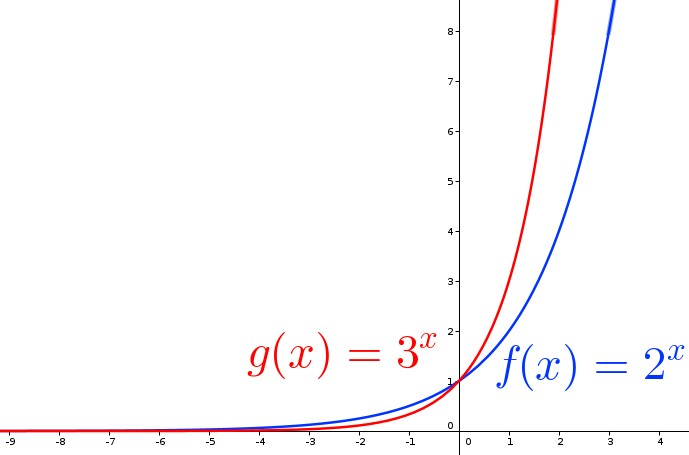
\includegraphics[scale=.5]{exponential.jpg}
\end{center}

The two functions overlap at \underline{$(0,1)$}.\\

The two graphs will not go below the line \underline{$y=0$}. This is called an \underline{\textbf{ASYMPTOTE}}. It is a way of describing the \underline{\textit{end behavior}} of the function. As the functions move towards negative infinity they will get smaller and smaller,  but they will never actually reach 0.\\

\pagebreak

\subsection{Translations}

A translation is when a function is moved around the graph. To move the graph up or down, add or subtract from the function.

\begin{center}
%\includegraphics[scale=.5]{transformation1.jpg} 
\end{center}

If there is no $+h$ on the back of the function, then the asymptote is at $y=0$. In these cases the $h$'s are $+2$ and $-1$.\\

If there is a $+h$ or $-h$ then the asymptote is at $\pm h$\\

\hrulefill

To move the function side to side add or subtract from the exponent. Be careful because it goes in the opposite direction of the sign. Notice the asymptote doesn't move\\

\begin{center}
%\includegraphics[scale=.5]{transformation2.jpg}
\end{center}

\pagebreak

\section{Method for Graphing}

\newcommand{\graph}{

\begin{tikzpicture}[scale=0.3]
   \tkzInit[xmax=10,ymax=10,xmin=-10,ymin=-10]
   \tkzGrid
   \tkzAxeXY
   
  \end{tikzpicture}
  }

Graph exponential equations. Easy method.

\begin{enumerate}
	\item Identify the asymptote. It's always the $\pm$ at the \textit{end} of the function
	
	\item Set the exponent equal to $0$
	
	\item Find the $y$ value when the exponent is equal to zero. Graph that point.
	
	\item Follow the asymtote until it passes through the point, and graph the exponentiality. \\
\end{enumerate}

\begin{multicols}{2}

\textbf{Example 1:} graph $y=2^{x-2}+3$\\

\graph

\textbf{Example 2:} graph $y=\left(\frac{1}{2} \right)^{x}-7$\\

\graph

\textbf{Example 3:} graph $y=-2^{x-2}+3$\\

\graph

\textbf{Example 4:} graph $y=2^{-x}-7$\\

\graph

\end{multicols}

\pagebreak

\textbf{You Try:} Graph the exponential Functions\\

\begin{multicols}{2}
 $y=3^x-5$\\

\graph

 $y=\left(\frac{1}{3} \right)^{x+4}+1$\\

\graph

$y= (-2)3^{x-1}+6$\\

\graph

$y= 3^{-x}$\\

\graph




\end{multicols}

\pagebreak

\section{Exponential Growth}

Compounding interest is an exponential expression because the exponent changes as time goes on. \\


$$A=P(1+r)^t \hspace{1cm}  A=P\left(1+\frac{r}{n}\right)^{nt}$$\\

$A=$ Actual amount -- what you'll end up with

$P=$ Principle -- original amount

$r=$ rate -- as a decimal, not as a fraction

$t=$ time\\

The \textit{independent} variable is $t$ the amount of time that goes by. The \textit{dependent} variable is $A$, the actual amount. This is because the actual amount depends on how much time goes by.\\ If we set this up as a relationship between $t$ and $A$, we would get an exponential function.

\hrulefill

\textbf{Example 1:}
How much will you have after investing \$500,000.00 compounded at 3\% for 12 years?\\


\vspace{1in}
\textbf{Example 2:}

Bacteria can multiply at an enormous rate when each cell doubles. If you get 3 bacteria cells on your hamburger and they double every hour, how much will be on your hamburger after 24 hours?\\

\vspace{1in}

\textbf{Example 3 -- You Try:}

In 1985, there were 102 cell phone subscribers in the small town of Stemville.  The number of subscribers increased by 55\% per year after 1985.  How many cell phone subscribers were in Stemville in 1994?

\pagebreak

\section{Exponential (radioactive) Decay}

Exponential decay is the same as exponential growth except for a minus sign.\\

$$A=P(1-r)^t \hspace{1cm}  A=P\left(1-\frac{r}{n}\right)^{nt}$$

We use this when something is decreasing in value.\\

\hrulefill

\textbf{Example 4:}\\
Each year the local country club sponsors a tennis tournament.  Play starts with 128 participants.  During each round, half of the players are eliminated.  How many players remain after 5 rounds?\\

\vspace{1in}

\textbf{Example 5:}\\
A radioactive isotope has a half-life of 1 day. If there was an original amount of 32 kilos of this isotope, how much would be left over after 15 days?\\

\vspace{1in}

\textbf{Example 6 -- You try:}\\
DDT is a toxic pesticide that was used in the 1970's. It is suspected to cause cancer in humans.  The half-life of DDT is about 15 years.  Half-life is the amount of time it takes for half of the amount of a substance to decay. If there was 100 grams of DDT on a certain plot of land, how much would be left over after 75 years?

\section{Exponential Growth -- NOTES}

Compounding interest is an exponential expression because the exponent changes as time goes on. \\


$A=$ 

$P=$ 

$r=$ 

$t=$ \\

The \textit{independent} variable is \underline{\hspace{1cm}} the amount of time that goes by. The \textit{dependent} variable is \underline{\hspace{1cm}}. This is because the actual amount \underline{\hspace{1cm}} on how much time goes by.\\ If we set this up as a relationship between $t$ and $A$, we would get an exponential function.

\hrulefill

\textbf{Example 1:}\\
How much will you have after investing \$500,000.00 compounded at 3\% for 12 years?\\


\vspace{1in}
\textbf{Example 2:}\\
Bacteria can multiply at an enormous rate when each cell doubles. If you get 3 bacteria cells on your hamburger and they double every hour, how much will be on your hamburger after 24 hours?\\

\vspace{1in}

\textbf{Example 3 -- You Try:}\\
In 1985, there were 102 cell phone subscribers in the small town of Stemville.  The number of subscribers increased by 55\% per year after 1985.  How many cell phone subscribers were in Stemville in 1994?

\pagebreak

\section{Exponential (radioactive) Decay -- NOTES}

Exponential decay is the same as exponential growth except for a \underline{\hspace{5cm}}.\\

$A=$\\

We use this when something is \underline{\hspace{5cm}} in value.\\

\hrulefill

\textbf{Example 4:}\\
Each year the local country club sponsors a tennis tournament.  Play starts with 128 participants.  During each round, half of the players are eliminated.  How many players remain after 5 rounds?\\

\vspace{1in}

\textbf{Example 5:}\\
A radioactive isotope has a half-life of 1 day. If there was an original amount of 32 kilos of this isotope, how much would be left over after 15 days?\\

\vspace{1in}

\textbf{Example 6 -- You try:}\\
DDT is a toxic pesticide that was used in the 1970's. It is suspected to cause cancer in humans.  The half-life of DDT is about 15 years.  Half-life is the amount of time it takes for half of the amount of a substance to decay. If there was 100 grams of DDT on a certain plot of land, how much would be left over after 75 years?

\section{The Number $e$}


e is an irrational number discovered by Leonhard Euler (pronounced oiler). It is commonly called Euler’s Number, but more commonly as the natural base. $e\approx 2.7182818...$ It is used as the base for many exponential functions, and has many applications in calculus.\\

$\mathbf{e}$ is calculated by the following expression as $n$ gets larger and larger $$\lim_{n \to \infty} \left(1+\frac{1}{n}\right)^n \approx 2.7182818$$\\

I hope this expression looks a little familiar.

\hrulefill

$e$ can be used a a regular exponential base. \\

So we can graph $y=e^x$\\

%source: https://en.wikipedia.org/wiki/Compound_interest#/media/File:Compound_Interest_with_Varying_Frequencies.svg
\begin{center}
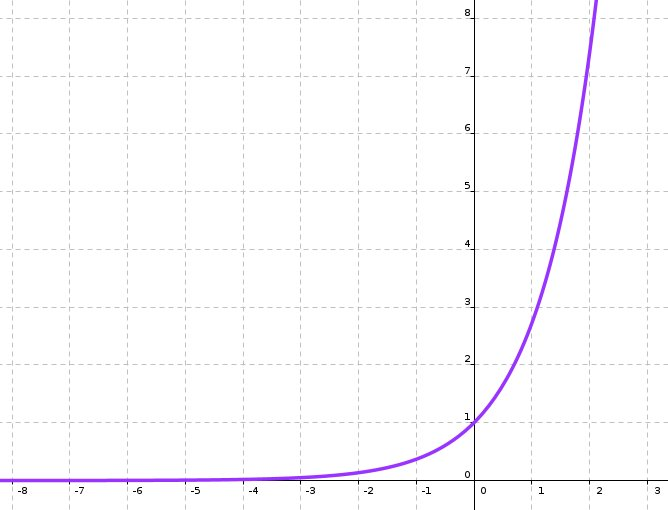
\includegraphics[scale=.75]{e.jpg}
\end{center}

What it comes down to is that $e$ is a number just like any other, and we can use it as such.\\

So what's so special about this number $e$?

\pagebreak

\section{Continuously Compounded Interest}

What is so special about $e$ is that we can compound interest continuously. The nice thing about that is that I get more money when interest is compounded more frequently.\\

\begin{center}
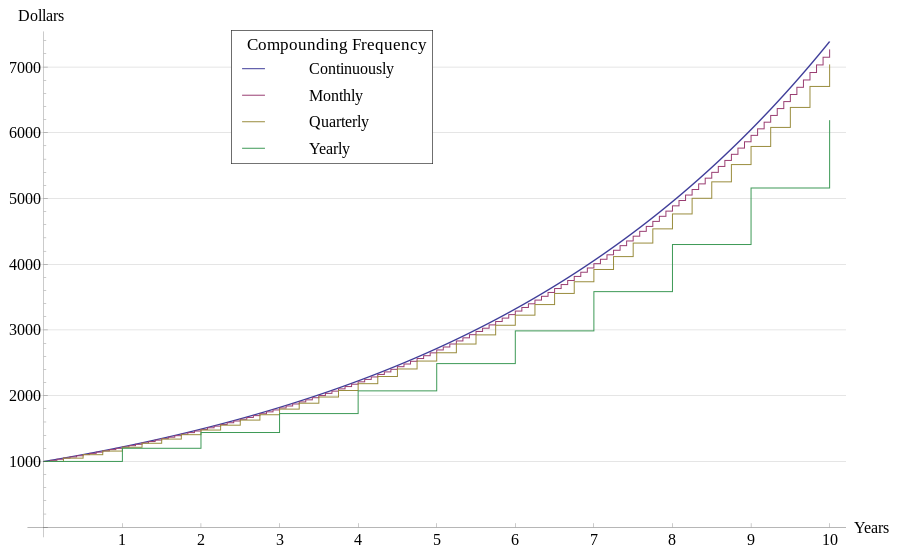
\includegraphics[scale=.5]{compoundinterest.png}
\end{center}

The graph above shows the same interest rate, but when the interest is compounded more often there are more significant gains made. \\

To calculate continuously compound interest we use the formula 

$$A=Pe^{rt}$$

Where\\
$A=$ Actualized amount\\
$P=$ Principal\\
$r=$ rate\\
$t=$ time\\

So basically all the letters are the same (remember $e$ is a number, not a variable), and it's a much tighter, neater package.\\

\pagebreak

\textbf{Example:} You deposit \$1500.00 in an account compound continuously at 3\%. How much will you have after 3 years?

\vspace{1in}

How much will you have after 10 years?\\

\vspace{1in}

How does this compare to compounded semi-annually (twice a year) for 10 years?\\

\vspace{1in}

\hrulefill

\textbf{Example 2:} How much will you have after investing \$2.00 compounded continuously since the year 1776?\\

\pagebreak

\section{Quiz Review}

Mr. Wolf \hfill NAME:\underline{\hspace{3in}}\\ 
wolf-math.com \hfill DATE:\underline{\hspace{2in}}\\


\begin{center}
	\begin{Large}
		 Graphing Exponentials \& Exponential Growth\\

	\end{Large}
	
		\textbf{Due Monday} 2014-10-13\\
\end{center}


\textbf{Graph the exponential function}\\

\begin{enumerate}[resume]
\begin{multicols}{2}

\item graph $y=2^{x-2}+3$\\

\graph

\item graph $y=\left(\frac{1}{2} \right)^{x}-7$\\

\graph

\item graph $y=-2^{x-2}+3$\\

\graph

\item  graph $y=2^{-x}-7$\\

\graph

\end{multicols}

\end{enumerate}

\hrulefill

\textbf{Compound the Interest}\\

$$A=P\left(1+\frac{r}{n}\right)^{n \cdot t}$$

\begin{enumerate}[resume]

\item How much money would you have after investing \$17 compounded daily at 10\% for 25 years?\\

\item (Population Growth) A rabbit population increases at 60\% compounded quarterly. If there were 20 rabbits to start with, how many rabbits will there be after 10 years?\\

\item 	\begin{enumerate}

			\item How much would you have after investing \$400 compounded monthly at 5\% for 10 years?\\

			\item How much would you have after investing \$400 compounded monthly at 5\% for 20 years?\\
			
			\item Even though twice as much time went by between (a) and (b), was twice as much money made?\\

		\end{enumerate} 

\end{enumerate}

\hrulefill

\textbf{Continuously Compound Interest}\\

$$A=Pe^{rt}$$

\begin{enumerate}[resume]

\item How much money will you have after investing \$600 compounded continuously at 4\% for 8 years?\\

\vspace{1cm}

\item 	\begin{enumerate}
		
			\item How much money will you have if you invest \$500 compounded continuously at 12\% for 10 years?\\
			
			\item What's the difference between (a) and if you compounded twice per year for 10 years.\\
			
		\end{enumerate}

\end{enumerate}

\pagebreak

\section{Quiz}

Mr. Wolf \hfill NAME:\underline{\hspace{3in}}\\ 
wolf-math.com \hfill DATE:\underline{\hspace{2in}}\\


\begin{center}
	\begin{Large}

		 Graphing Exponentials \& Exponential Growth\\

	\end{Large}
	
		\textbf{OPEN NOTE} \\
\end{center}


\textbf{Graph the exponential function}\\

\begin{enumerate}[resume]
\begin{multicols}{2}

\item graph $y=2^{x+2}-3$\\

\graph

\item graph $y=\left(\frac{1}{2} \right)^{x}-8$\\

\graph

\item graph $y=-2^{x+5}-3$\\

\graph

\item  graph $y=2^{-x}+5$\\

\graph

\end{multicols}

\end{enumerate}

\hrulefill

\textbf{Compound the Interest}\\

$$A=P\left(1+\frac{r}{n}\right)^{n \cdot t}$$

\begin{enumerate}[resume]

\item How much money would you have after investing \$17 compounded daily at 10\% for 25 years?\\

\item (Population Growth) A rabbit population increases at 60\% compounded quarterly. If there were 20 rabbits to start with, how many rabbits will there be after 10 years?\\

\item 	\begin{enumerate}

			\item How much would you have after investing \$1000 compounded monthly at 6\% for 10 years?\\

			\item How much would you have after investing \$1000 compounded monthly at 6\% for 30 years?\\
			
			\item Even though triple the time went by between (a) and (b), was triple the money made?\\

		\end{enumerate} 

\end{enumerate}

\hrulefill

\textbf{Continuously Compound Interest}\\

$$A=Pe^{rt}$$

\begin{enumerate}[resume]

\item How much money will you have after investing \$800 compounded continuously at 4\% for 6 years?\\

\vspace{1cm}

\item 	\begin{enumerate}
		
			\item How much money will you have if you invest \$1200 compounded continuously at 10\% for 14 years?\\
			
			\item What's the difference between (a) and compounded twice per year for 14 years.\\
			
		\end{enumerate}

\end{enumerate}

\vspace{1cm}

**Now you're done :-)
\end{document}